\documentclass[10pt]{article}
\usepackage[letterpaper,margin=0.8in]{geometry}
\usepackage{amsmath,amssymb,booktabs,tabularx,microtype,xcolor,graphicx,longtable,array}
\usepackage[colorlinks,allcolors=blue!55!black]{hyperref}
\setlength{\parindent}{0pt}\setlength{\parskip}{5pt}
\begin{document}
{\small\scshape Public human ratings \quad|\quad Does CE-fitting beat Pearson-fitting on real rating data, and from how many ratings?}\par
{\LARGE\bfseries Break-even number of human ratings: CE-fit vs Pearson-fit on real public rating sets}\par
{\small As of 11-23-2026 \quad|\quad \href{https://github.com/brando90/judges-dont-need-psychometrics-or-corr/tree/main/experiments/28_public_rating_sets_chaosnli_dices_frontier_judges_ce_vs_pearson_start_23Nov2026}{Experiment 28, code, forecasts and tables}}\par
\textbf{Bottom line.} On five public sets of real human ratings (ChaosNLI SNLI and MNLI-m, an alphaNLI control, DICES-350 and DICES-990) and five frontier judges, fitting the judge by cross-entropy (CE) beat fitting it by Pearson correlation and beat the uniform forecast on held-out ranked probability score (RPS) after only 4 to 8 human ratings at one rating per item, or 10 to 20 ratings at five per item, in all 25 set-by-judge cells. At \$5 a rating that is under \$100. Scored on RPS, CE and total variation, never on correlation, the Pearson-fit judge was significantly better in 19 of 325 comparison cells, mostly at two training items, where the tie rule keeps the raw judge. Two findings limit the claim. (1) The raw frontier judge is already strong on ChaosNLI: CE-fit beats it, sustained, only from 16 to 32 ratings on MNLI-m (three of five judges), 64 on SNLI (one judge) and 256 on alphaNLI (one judge), and from 8 to 128 on DICES-350 and 16 on DICES-990 (four judges). For the remaining judge-set pairs it never does within 256. (2) Pearson-fit followed by a distribution calibration on the same ratings (a rank-then-calibrate recipe) is worse than CE-fit on SNLI and alphaNLI, level with it on MNLI-m at 256 ratings and better than it on DICES from 64 ratings on (a few judges); so what helps is fitting a distribution with a proper score, not the correlation step. ChaosNLI SNLI and MNLI-m are subsets chosen for human disagreement, so these break-even sizes may not carry to easier items.

\textbf{What each metric can and cannot see.} Pearson and Spearman see only the order and linear scale of the expected score: the first moment, up to level and scale (R1). RPS, CE and TVD see the whole forecast distribution against the human distribution (R2). Top-1 agreement sees only the mode. Ordinal coding is an assumption (NLI: contradiction $<$ neutral $<$ entailment; DICES: No $<$ Unsure $<$ Yes); CE and TVD do not depend on it, RPS and Pearson do.

\section*{1. Derivation}
\textbf{R1. Pearson sees only the first moment, up to level and scale.} For a forecast $q_x$ over categories with scores $s_k$, the expected score is $m_q(x)=\sum_k s_k q_x(k)$. Pearson correlation of $m_q(X)$ with the human mean $\mu(X)$ satisfies $\operatorname{Corr}(a+b\,m_q,\mu)=\operatorname{Corr}(m_q,\mu)$ for every $a$ and every $b>0$. Two judges whose expected scores differ by such a map get the same score whatever their spread, skew or calibration. With $K$ categories the map $q\mapsto m_q$ discards $K-2$ degrees of freedom of the forecast, and a fit that maximizes this correlation cannot choose among forecasts with equal $m_q$. Here the fit chooses among 27 transforms $q\propto p^t\exp(bu_k+cu_k^2)$; transforms that change the level or scale of $m_q$ are invisible to the objective, so which one it picks is decided by noise in the training means.

\textbf{R2. CE and RPS are proper; they are minimized only by the full human distribution.} For true distribution $h$ and forecast $q$, $\mathrm{CE}(q)-\mathrm{CE}(h)=D_{\mathrm{KL}}(h\Vert q)\ge0$ with equality only at $q=h$. The ranked probability score $\mathrm{RPS}(q,y)=\frac1{K-1}\sum_{k<K-1}(F_q(k)-\mathbf 1[y\le k])^2$ is the sum of Brier scores of the $K-1$ cumulative events, so its expectation is minimized at $F_q=F_h$, again only at $q=h$. Both therefore reward getting the mean and every higher moment right, and neither is defined through correlation. TVD$=\tfrac12\sum_k|h_k-q_k|$ is a metric on distributions, zero only at $q=h$.

\textbf{R3. Non-circular evaluation.} Every test item is scored against its full empirical human distribution (100, 123 or 69 to 76 ratings), so mean test CE and RPS equal means over individual held-out human ratings. Pearson and Spearman are computed for description only. Top-1 agreement is reported because neither objective optimizes it.

\textbf{R4. Break-even.} Let $\Delta_B$ be the mean over test items of (comparator metric minus CE-fit metric) at budget $B$ ratings, positive when CE-fit is better, averaged over 200 training draws. The simultaneous lower bound $L_B=\bar\Delta_B-c\,\widehat{\mathrm{se}}_B$ takes $c$ as the 97.5\% quantile of the maximum standardized bootstrap deviation across the budgets of one condition. The break-even $N^\star=\min\{B: L_{B'}>0\ \text{for all tested } B'\ge B\}$, and for the two primary comparators (Pearson-fit and uniform) both bounds must exceed zero. It is the smallest tested budget, not an interpolation.

\textbf{R5. The alphaNLI control.} With $K=2$ the mean $m_q=q(1)$ identifies $q$, so R1 removes no shape information. If CE-fit still beats Pearson-fit there, the gap comes from level and scale, which R1 shows Pearson cannot see, and not from higher moments. It does (Table 1).


\section*{2. Design}
Data: public files read in full, per-item human count vectors. Items run: ChaosNLI SNLI 600 of 1,514, MNLI-m 600 of 1,599, alphaNLI 400 of 1,532, DICES-350 350 of 350, DICES-990 400 of 990 (seeded subsamples, protocol frozen before any judge call). 
Judges (harness: Stanford AI API Gateway chat completions, temperature 0, 2,048 output tokens, one call per item): GPT-6 Astra and Claude Opus 5.5 (closed weights); Kimi K3, GLM 5.3 and DeepSeek V4.1 Flash (open weights). Orchestration and analysis: Claude Sonnet 5.5 in Claude Code, headless. 
Each forecast goes through the 27-transform head of experiment 21, fitted by CE (training CE on individual ratings), by Pearson (correlation of expected score with the training item mean), by RPS (extra), or not fitted (raw). Comparators fitted from the same ratings: uniform, training histogram, Pearson-fit then four-bin distribution calibration. 
Budgets: 4 to 256 ratings at one per item; 10 to 320 at five per item; five folds, 200 training draws per fold, nested budgets, 4,000 item bootstraps. Forecasts, receipts and costs were committed before any label was joined; an independent plain-loop re-implementation reproduced the vectorized scores to $10^{-15}$ for three judge-set pairs.

\section*{3. Results}
\textbf{Table 1. Break-even $N^\star$ on held-out RPS, one rating per item (range over the 5 judges; ``none'' = no sustained win).}\par
\footnotesize
\begin{tabular}{lllllll}\toprule
Set & vs Pearson-fit & vs uniform & vs both & vs histogram & vs Pearson+calibration & vs raw judge \\ \midrule
ChaosNLI SNLI & 4 & 4 & 4 & 4 & 4 & 64 (4/5 none) \\
ChaosNLI MNLI-m & 4 & 4 & 4 & 4 & none (5/5) & 16-32 (2/5 none) \\
ChaosNLI alphaNLI (control) & 4-8 & 4 & 4-8 & 4 & 4 (1/5 none) & 256 (4/5 none) \\
DICES-350 & 4 & 8 & 8 & 16-256 (3/5 none) & 8 (4/5 none) & 8-128 \\
DICES-990 & 4 & 4 & 4 & 8-64 & none (5/5) & 16 (1/5 none) \\
\bottomrule\end{tabular}


\textbf{Table 2. Same, five ratings per item (N is total ratings).}\par
\footnotesize
\begin{tabular}{lllllll}\toprule
Set & vs Pearson-fit & vs uniform & vs both & vs histogram & vs Pearson+calibration & vs raw judge \\ \midrule
ChaosNLI SNLI & 20 & 10 & 20 & 10 & 10 & 80 (4/5 none) \\
ChaosNLI MNLI-m & 20 & 10 & 20 & 10 & none (5/5) & 20-80 (2/5 none) \\
ChaosNLI alphaNLI (control) & 20 & 10 & 20 & 10 & 10 & 320 (4/5 none) \\
DICES-350 & 10-20 & 10-20 & 10-20 & 20-160 (3/5 none) & 20 (4/5 none) & 10-160 \\
DICES-990 & 20 & 10 & 20 & 10-80 & none (5/5) & 20-40 (1/5 none) \\
\bottomrule\end{tabular}


\textbf{Table 3. Mean held-out RPS over the 5 judges, one rating per item; left block 16 ratings, right block 256 ratings (lower is better).}\par
\footnotesize
\begin{tabular}{lrrrrrrrrrrrr}\toprule
Set & raw & unif & hist & Pear & Pear+cal & CE & raw & unif & hist & Pear & Pear+cal & CE \\ \midrule
ChaosNLI SNLI & 0.117 & 0.196 & 0.199 & 0.150 & 0.148 & 0.128 & 0.117 & 0.196 & 0.190 & 0.134 & 0.124 & 0.115 \\
ChaosNLI MNLI-m & 0.170 & 0.213 & 0.211 & 0.203 & 0.186 & 0.174 & 0.170 & 0.213 & 0.201 & 0.185 & 0.161 & 0.163 \\
ChaosNLI alphaNLI (control) & 0.121 & 0.250 & 0.263 & 0.155 & 0.151 & 0.133 & 0.121 & 0.250 & 0.250 & 0.125 & 0.126 & 0.120 \\
DICES-350 & 0.253 & 0.267 & 0.241 & 0.293 & 0.250 & 0.242 & 0.253 & 0.267 & 0.230 & 0.276 & 0.221 & 0.226 \\
DICES-990 & 0.222 & 0.269 & 0.224 & 0.261 & 0.225 & 0.216 & 0.222 & 0.269 & 0.213 & 0.261 & 0.194 & 0.198 \\
\bottomrule\end{tabular}

\textbf{Table 4. The other metrics at 256 ratings (one per item), mean over judges: CE in nats, TVD, top-1 agreement. CE-fit is better on all three on every set except top-1 on alphaNLI (0.878 against 0.885).}\par
\footnotesize
\begin{tabular}{lrrrrrr}\toprule
Set & Pearson CE & Pearson TVD & Pearson top-1 & CE-fit CE & CE-fit TVD & CE-fit top-1 \\ \midrule
ChaosNLI SNLI & 0.824 & 0.235 & 0.715 & 0.713 & 0.169 & 0.813 \\
ChaosNLI MNLI-m & 1.037 & 0.261 & 0.606 & 0.911 & 0.208 & 0.662 \\
ChaosNLI alphaNLI (control) & 0.454 & 0.131 & 0.885 & 0.396 & 0.125 & 0.878 \\
DICES-350 & 1.272 & 0.314 & 0.621 & 0.851 & 0.163 & 0.797 \\
DICES-990 & 1.047 & 0.315 & 0.565 & 0.757 & 0.138 & 0.852 \\
\bottomrule\end{tabular}

\textbf{Table 5. Every comparator that is significantly better than CE-fit on RPS (cells are judge-by-budget-by-condition combinations; 65 per set).} Pearson-fit at 10 ratings is the two-item, five-ratings condition, where almost every transform gets Pearson $\pm1$, so the tie rule keeps the identity, that is the raw judge; the raw judge beats a head fitted from two items.\par
\scriptsize
\begin{tabular}{llrlp{3.4in}}\toprule
Comparator better than CE-fit & Set & Cells & Budgets & Judges \\ \midrule
Pearson-fit & ChaosNLI SNLI & 5 of 65 & 10 to 10 & Claude Opus 5.5, DeepSeek V4.1 Flash, GLM 5.3, GPT-6 Astra, Kimi K3 \\
Pearson-fit & ChaosNLI MNLI-m & 5 of 65 & 10 to 10 & Claude Opus 5.5, DeepSeek V4.1 Flash, GLM 5.3, GPT-6 Astra, Kimi K3 \\
Pearson-fit & ChaosNLI alphaNLI (control) & 6 of 65 & 4 to 10 & Claude Opus 5.5, DeepSeek V4.1 Flash, GLM 5.3, GPT-6 Astra, Kimi K3 \\
Pearson-fit & DICES-350 & 1 of 65 & 10 to 10 & Claude Opus 5.5 \\
Pearson-fit & DICES-990 & 2 of 65 & 10 to 10 & Claude Opus 5.5, GLM 5.3 \\
raw judge & ChaosNLI SNLI & 51 of 65 & 4 to 320 & Claude Opus 5.5, DeepSeek V4.1 Flash, GLM 5.3, GPT-6 Astra, Kimi K3 \\
raw judge & ChaosNLI MNLI-m & 33 of 65 & 4 to 320 & Claude Opus 5.5, DeepSeek V4.1 Flash, GLM 5.3, GPT-6 Astra, Kimi K3 \\
raw judge & ChaosNLI alphaNLI (control) & 50 of 65 & 4 to 320 & Claude Opus 5.5, DeepSeek V4.1 Flash, GLM 5.3, GPT-6 Astra, Kimi K3 \\
raw judge & DICES-350 & 9 of 65 & 4 to 40 & Claude Opus 5.5, GLM 5.3, Kimi K3 \\
raw judge & DICES-990 & 13 of 65 & 4 to 40 & Claude Opus 5.5, DeepSeek V4.1 Flash, GLM 5.3, GPT-6 Astra, Kimi K3 \\
histogram & DICES-350 & 7 of 65 & 4 to 160 & DeepSeek V4.1 Flash, Kimi K3 \\
Pearson+calibration & ChaosNLI MNLI-m & 3 of 65 & 256 to 320 & DeepSeek V4.1 Flash, Kimi K3 \\
Pearson+calibration & DICES-350 & 12 of 65 & 64 to 320 & DeepSeek V4.1 Flash, GPT-6 Astra \\
Pearson+calibration & DICES-990 & 10 of 65 & 64 to 320 & DeepSeek V4.1 Flash, GPT-6 Astra, Kimi K3 \\
RPS-fit (extra) & DICES-350 & 13 of 65 & 32 to 320 & DeepSeek V4.1 Flash, GPT-6 Astra \\
RPS-fit (extra) & DICES-990 & 3 of 65 & 10 to 320 & GPT-6 Astra \\
\bottomrule\end{tabular}

\textbf{Table 6. Cross-set break-even. Codex's thresholds are as published in experiments 23 to 25 and were not re-run; their definitions of the Pearson comparator differ in detail.} n.r. = not reported there.\par
\scriptsize
\begin{tabular}{p{2.1in}p{1.0in}p{1.4in}p{0.9in}p{1.4in}}\toprule
Set & Setting & CE beats Pearson from N = & CE beats uniform from N = & CE beats Pearson+calibration from N = \\ \midrule
ChaosNLI SNLI, MNLI-m, alphaNLI (this experiment) & 5 judges, one rating per item & 4 to 8 & 4 & SNLI 4; MNLI-m none; alphaNLI 4 (one judge none) \\
DICES-350, DICES-990 (this experiment) & 5 judges, one rating per item & 4 & 4 to 8 & DICES-350 8 (4 of 5 judges none); DICES-990 none \\
KonIQ-10k (Codex, exp. 23) & image quality & 12 (24 with draw resampling, 48 at three per image) & 12 & no budget beats all four controls \\
USR PersonaChat (Codex, exp. 23) & dialogue quality & 48 (96 at three grades per response) & 48 & n.r. \\
USR Topical-Chat (Codex, exp. 23) & dialogue quality & none & none & n.r. \\
MovieLens 100K (Codex, exp. 23) & movie stars & CE beats Pearson at all budgets & none & none \\
SummEval, GPT-4 forecasts (Codex, exp. 23) & summary quality & no sustained CE win at 6 to 768 ratings & none & calibrated Pearson and histogram beat CE \\
HelpSteer2 LoRA Qwen3-4B (Codex, exp. 24 and 25) & fine-tuned judge & n.r. & from 16 total ratings & calibrated Pearson: none up to 8,192 \\
HelpSteer2 LoRA Llama-3.1-8B (Codex, exp. 24 and 25) & fine-tuned judge & n.r. & none & none \\
\bottomrule\end{tabular}

\textbf{Table 7. What N ratings cost (USD), under four per-rating prices.} Observed: ChaosNLI paid up to \$0.50 per batch of ten examples; Chaganty et al. about \$0.15 per summary judgment. Illustrative: \$1 and \$5 (assumptions). DICES and HelpSteer2 prices could not be established from public sources.\par
\footnotesize
\begin{tabular}{rrrrr}\toprule
N ratings & \$0.05 & \$0.15 & \$1 & \$5 \\ \midrule
8 & 0.40 & 1.20 & 8.00 & 40.00 \\
20 & 1.00 & 3.00 & 20.00 & 100.00 \\
64 & 3.20 & 9.60 & 64.00 & 320.00 \\
256 & 12.80 & 38.40 & 256.00 & 1,280.00 \\
1000 & 50.00 & 150.00 & 1,000.00 & 5,000.00 \\
\bottomrule\end{tabular}

Reading Table 7 with Tables 1 and 2: beating Pearson-fit and uniform takes 4 to 8 ratings (one per item) or 10 to 20 (five per item), at most about \$100 at \$5 a rating. Beating the raw judge takes 16 to 256 ratings ($\approx$\$80 to \$1,280 at \$5) where it happens, and on SNLI, alphaNLI and some judges it does not within 256.

\textbf{Table 8. Forecast validity and judge-call cost (list rate for the closed judges; the open models are listed at 0 and are also shown at a 1.4/4.4 stand-in).} Fallback means unparseable or failed output, scored as uniform by a rule frozen before the run; none of the 11,750 calls errored. Estimated total \$19.69 at configured rates (\$39.0 with the 1.4/4.4 stand-in for the open models), plus \$1.34 in the layer 4 task: under the \$80 stop of the shared \$100 cap.\par
\footnotesize
\begin{tabular}{lrrrrrr}\toprule
Judge & Uniform fallback & Calls ok & Input tokens & Output tokens & USD configured & USD stand-in \\ \midrule
Claude Opus 5.5 & 41 of 2350 & 2350 & 699,281 & 205,401 & 6.91 & 1.88 \\
DeepSeek V4.1 Flash & 139 of 2350 & 2350 & 522,230 & 1,252,039 & 0.00 & 6.24 \\
GLM 5.3 & 54 of 2350 & 2350 & 474,355 & 1,395,108 & 0.00 & 6.80 \\
GPT-6 Astra & 0 of 2350 & 2350 & 461,981 & 163,230 & 12.78 & 1.36 \\
Kimi K3 & 168 of 2350 & 2350 & 516,466 & 1,258,030 & 0.00 & 6.26 \\
\bottomrule\end{tabular}

\begin{center}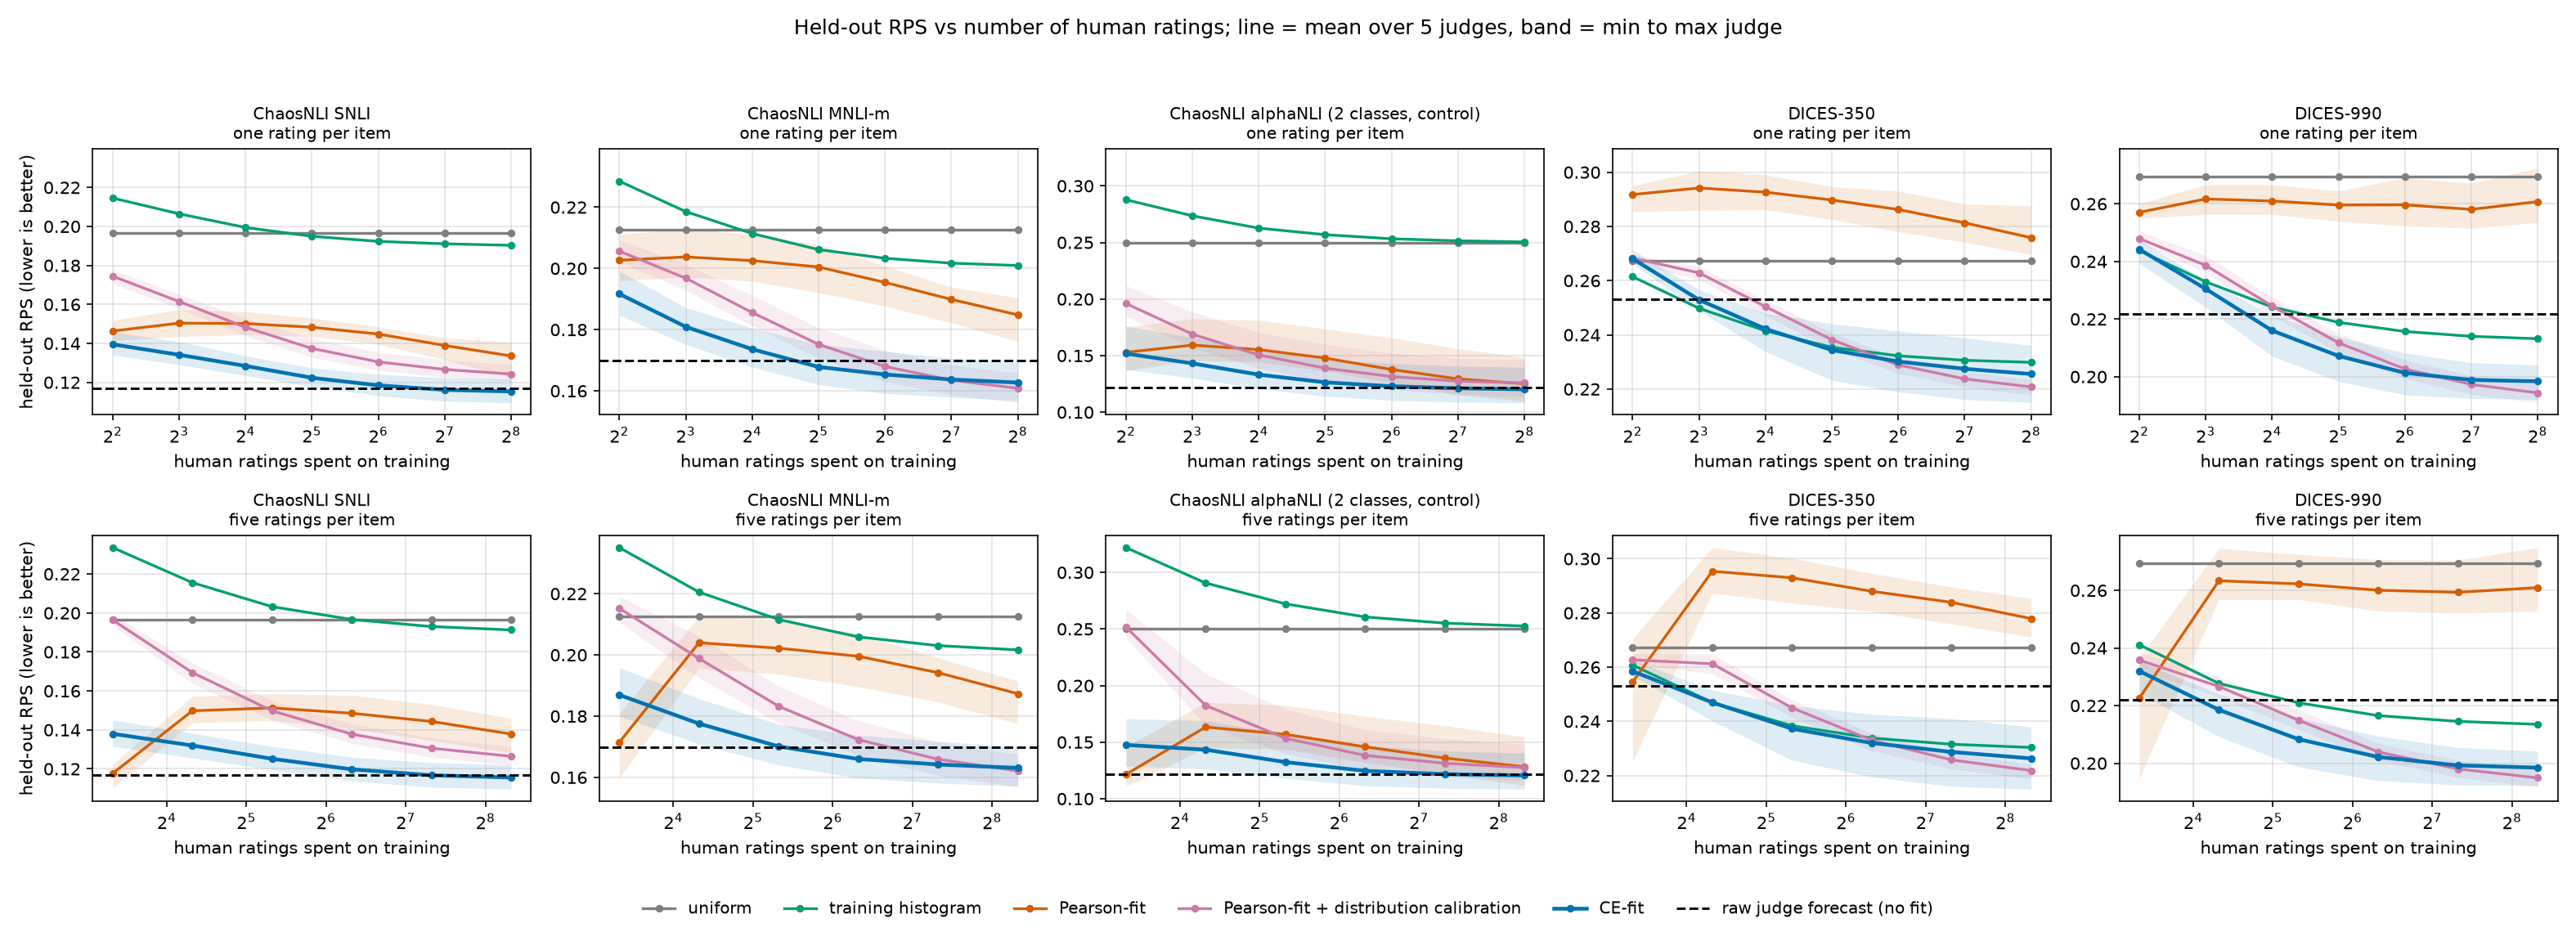
\includegraphics[width=\linewidth]{../figures/learning_curves_rps.png}\end{center}
\textbf{Figure 1.} Held-out RPS against ratings spent; band is min to max over judges.

\begin{center}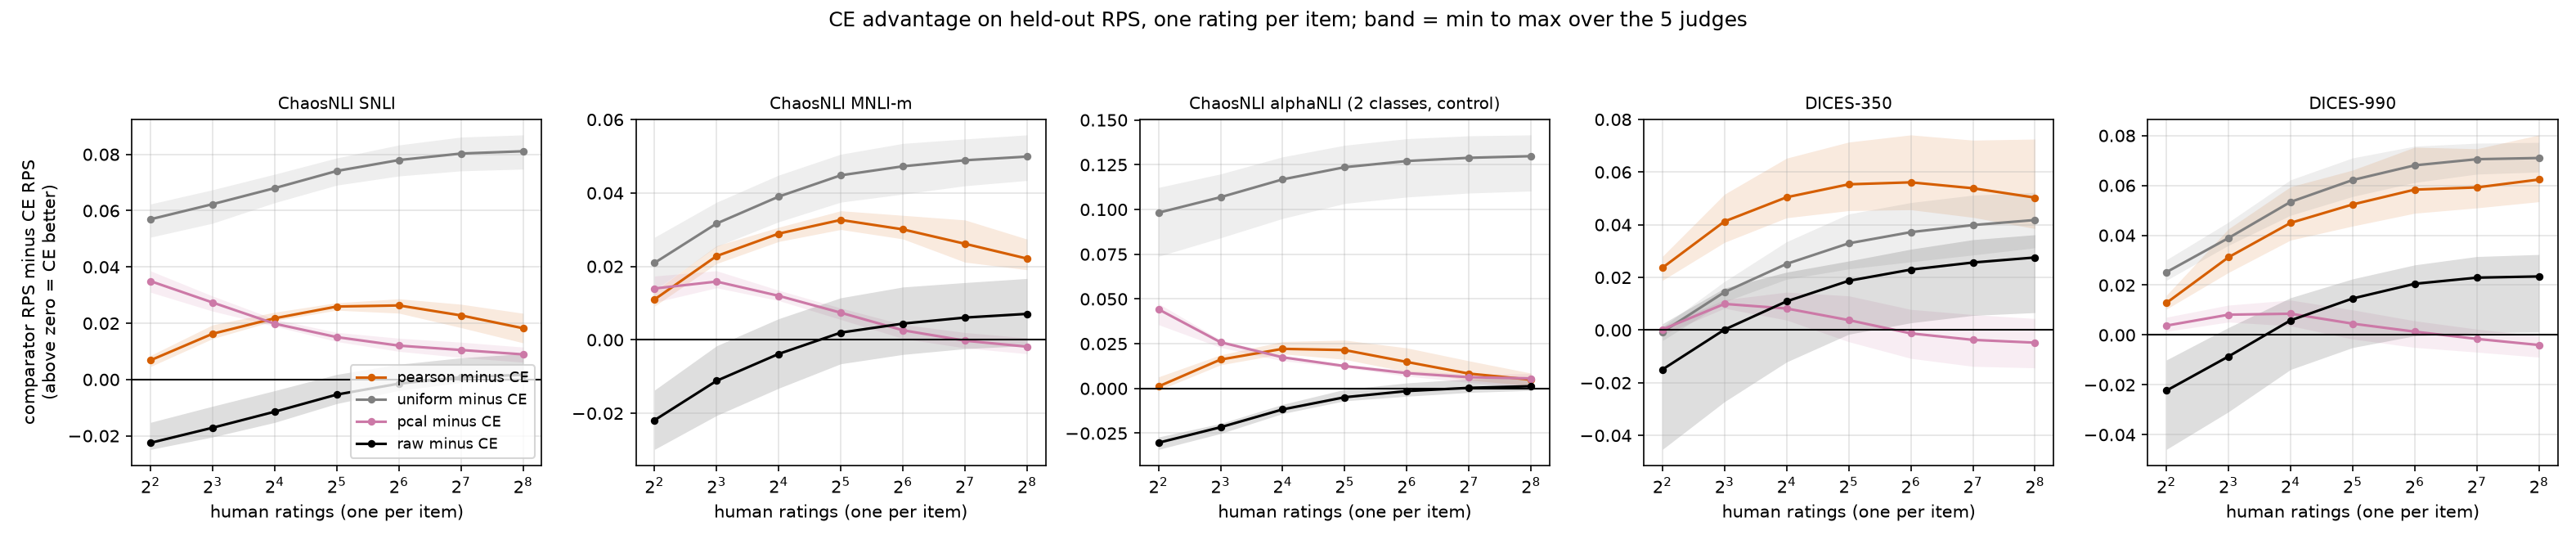
\includegraphics[width=\linewidth]{../figures/ce_advantage_rps_d1.png}\end{center}
\textbf{Figure 2.} CE advantage over each comparator, one rating per item; above zero is CE better.

\section*{4. Caveats}
\begin{itemize}\setlength\itemsep{1pt}
\item Ordinal coding is assumed (R1, Design); alphaNLI has two categories and is a control, not a test of shape.
\item ChaosNLI SNLI and MNLI-m keep only items whose original five labels were not unanimous (agree\_3), so they over-represent disagreement; DICES items are adversarial conversations. Break-even sizes may differ on easier items.
\item Ratings here are drawn from 100, 123 or about 73 released ratings per item; test scores condition on that pool, on the item subsample and on the 200 draws.
\item Frozen parsing turned 0 to 7\% of each judge's outputs into the uniform forecast (Table 8; Claude Opus 5.5 often put prose before the JSON). No lenient re-parse was run.
\item Intervals for the raw-judge comparison are the same simultaneous bootstrap; break-even ``vs raw'' compares a fitted head with an unfitted forecast, so it is the practical question, not the correlation-versus-CE question.
\item Pearson-fit here selects among the same 27 transforms as CE-fit; a different Pearson-trained model (for example fine-tuned weights) is not tested, only head fitting (experiments 24 and 25 cover weights).
\item Per-rating prices come from other studies and assumptions (Table 7); no payment was made here.
\item The catalog (next pages) lists 26 sets. Not verified: Jigsaw Unintended Bias (login wall); Chatbot Arena file contents (gated; card only); WebGPT beyond a 2,752-pair sample; SHP beyond 6 of 18 subreddits; licences and selection for LeWiDi-2025 and Pavlick and Kwiatkowski. Only ChaosNLI and DICES were run here; Codex covered KonIQ, SummEval, USR, MovieLens and HelpSteer2.
\end{itemize}

\clearpage\newgeometry{paperwidth=11in,paperheight=8.5in,margin=0.5in}\pdfpagewidth=11in\pdfpageheight=8.5in
\section*{Appendix. Catalog of public rating sets (checked at the source, 11-23-2026)}
\tiny\setlength{\tabcolsep}{2pt}
\begin{longtable}{@{}r p{1.15in} p{1.0in} p{0.75in} p{0.8in} p{0.8in} p{0.9in} p{0.8in} p{1.2in} p{1.5in}@{}}
\toprule \# & Name & Task & Items & Ratings per item (min / median / max) & Scale & Individual ratings released & Licence & Link & Selection bias \\ \midrule\endhead
1 & ChaosNLI (SNLI, MNLI-m, alphaNLI parts) & NLI label distribution & 1,514 + 1,599 + 1,532 = 4,645 & 100 / 100 / 100 & 3 classes (alphaNLI: 2) & per-item counts only, no rater ids & CC BY-NC 4.0 & \href{https://github.com/easonnie/ChaosNLI}{github.com/\allowbreak{}easonnie/\allowbreak{}ChaosNLI} & SNLI and MNLI-m: only items whose original 5 labels had 3-of-5 agreement (biased toward disagreement); alphaNLI is the full dev set \\
2 & DICES-350 & safety rating of adversarial chatbot conversations & 350 & 123 / 123 / 123 & Yes (unsafe) / No / Unsure & yes, with rater ids and demographics & CC BY 4.0 & \href{https://github.com/google-research-datasets/dices-dataset/tree/main/350}{github.com/\allowbreak{}google-\allowbreak{}research-\allowbreak{}datasets/\allowbreak{}dices-\allowbreak{}dataset/\allowbreak{}tree/\allowbreak{}main/\allowbreak{}} & adversarial conversations, stratified toward clear safe/unsafe gold labels \\
3 & DICES-990 & same & 990 & 69 / 73 / 76 & Yes / No / Unsure & yes, 172 raters, with demographics & CC BY 4.0 & \href{https://github.com/google-research-datasets/dices-dataset/tree/main/990}{github.com/\allowbreak{}google-\allowbreak{}research-\allowbreak{}datasets/\allowbreak{}dices-\allowbreak{}dataset/\allowbreak{}tree/\allowbreak{}main/\allowbreak{}} & adversarial conversations, stratified by adversariality group \\
4 & HelpSteer2 (+ disagreements file) & helpfulness etc. of LLM replies & 21,362 & 2 / 3 / 6 & 5 attributes, integers 0-4 & yes (lists, no rater ids) & CC BY 4.0 & \href{https://huggingface.co/datasets/nvidia/HelpSteer2}{huggingface.co/\allowbreak{}datasets/\allowbreak{}nvidia/\allowbreak{}HelpSteer2} & ShareGPT prompts; train/val keeps only samples with limited annotator spread \\
5 & MT-Bench human judgments & pairwise model preference & 1,814 pairs (3,355 votes) & 1 / 2 / 7 & model\_a / model\_b / tie & yes, 65 pseudonymous judges & CC BY 4.0 & \href{https://huggingface.co/datasets/lmsys/mt_bench_human_judgments}{huggingface.co/\allowbreak{}datasets/\allowbreak{}lmsys/\allowbreak{}mt\_bench\_human\_judgments} & 80 hand-built questions, 6 models, volunteer graduate-student judges \\
6 & SummEval & summary quality (4 dimensions) & 1,600 summaries & 8 / 8 / 8 (3 expert + 5 crowd) & Likert 1-5 & yes, no rater ids & no data licence stated (repo MIT) & \href{https://github.com/Yale-LILY/SummEval}{github.com/\allowbreak{}Yale-\allowbreak{}LILY/\allowbreak{}SummEval} & 100 random CNN/DM articles, 16 systems; MTurk workers with high approval \\
7 & KonIQ-10k & image quality & 10,073 & 93 / 106 / 157 & 5-point ACR & per-image histogram only & CC BY 4.0 with per-image exceptions & \href{https://database.mmsp-kn.de/koniq-10k-database.html}{database.mmsp-\allowbreak{}kn.de/\allowbreak{}koniq-\allowbreak{}10k-\allowbreak{}database.html} & tag-sampled Creative-Commons YFCC100M images \\
8 & USR (Topical-Chat, PersonaChat) & dialogue response quality & 660 & 3 / 3 / 3 & per quality: 0-1, 1-3, 1-5 & yes, partly with annotator ids & none stated (code Apache-2.0) & \href{http://shikib.com/usr}{http:/\allowbreak{}/\allowbreak{}shikib.com/\allowbreak{}usr} & 60 + 60 random contexts, six responses each \\
9 & Stanford Sentiment Treebank raw & phrase sentiment & 239,232 phrases & 3 / 3 / 6 & slider 1-25 & yes (raw scores) & none stated & \href{https://nlp.stanford.edu/sentiment/}{nlp.stanford.edu/\allowbreak{}sentiment/\allowbreak{}} & Rotten Tomatoes snippets, MTurk \\
10 & MovieLens 100K & movie ratings & 1,682 movies & 1 / 27 / 583 & 1-5 stars & yes, user ids & research-use terms & \href{https://grouplens.org/datasets/movielens/100k/}{grouplens.org/\allowbreak{}datasets/\allowbreak{}movielens/\allowbreak{}100k/\allowbreak{}} & self-selected raters, users with at least 20 ratings \\
11 & Chatbot Arena Conversations & pairwise vote, in the wild & 33,000 conversations & 1 (n.v. in file; gated, card only) & winner field & yes per card (n.v. in file), anonymised user id & prompts CC BY 4.0, outputs CC BY-NC 4.0 (gated) & \href{https://huggingface.co/datasets/lmsys/chatbot_arena_conversations}{huggingface.co/\allowbreak{}datasets/\allowbreak{}lmsys/\allowbreak{}chatbot\_arena\_conversations} & self-selected hobbyist volunteers \\
12 & WebGPT comparisons & pairwise comparison of answers & 19,578 & 1 (count from a 2,752-pair sample; labelers per pair n.v.) & score -1 to 1 & no per-labeler ratings & none stated & \href{https://huggingface.co/datasets/openai/webgpt_comparisons}{huggingface.co/\allowbreak{}datasets/\allowbreak{}openai/\allowbreak{}webgpt\_comparisons} & 98\% ELI5 questions, 10 Upwork + few labelers \\
13 & SHP & which Reddit reply is preferred & 385,563 pairs & aggregate net scores only & score\_A, score\_B & no individual votes & Reddit-terms statement only & \href{https://huggingface.co/datasets/stanfordnlp/SHP}{huggingface.co/\allowbreak{}datasets/\allowbreak{}stanfordnlp/\allowbreak{}SHP} & popular subreddits, top-scoring posts \\
14 & WMT MQM (newstest2020 en-de, zh-en) & translation error annotation & 14,180 + 20,000 & 3 / 3 / 3 & error spans with severity & yes, rater ids rater1-6 & Apache-2.0 & \href{https://github.com/google/wmt-mqm-human-evaluation}{github.com/\allowbreak{}google/\allowbreak{}wmt-\allowbreak{}mqm-\allowbreak{}human-\allowbreak{}evaluation} & top-performing systems plus a few chosen ones \\
15 & CIFAR-10H & 10-way image classification & 10,000 & 47 / 51 / 63 (counts file) & 10 classes & counts file; raw CSV with annotator ids & CC BY-NC-SA 4.0 & \href{https://github.com/jcpeterson/cifar-10h}{github.com/\allowbreak{}jcpeterson/\allowbreak{}cifar-\allowbreak{}10h} & CIFAR-10 test images; MTurk workers passing a 75\% attention check \\
16 & oasst1 & message quality labels & 161,443 messages (148,855 labelled) & 1 / 3 / 13 labels per message & aggregate mean and count per label & no (aggregates only) & Apache-2.0 & \href{https://huggingface.co/datasets/OpenAssistant/oasst1}{huggingface.co/\allowbreak{}datasets/\allowbreak{}OpenAssistant/\allowbreak{}oasst1} & unpaid volunteers recruited mainly via Discord \\
17 & Wikipedia Detox: toxicity & comment toxicity & 159,686 & 8 / 10 / 21 & 5-point ordinal (+ binary) & yes, rater ids & CC0 & \href{https://figshare.com/articles/dataset/Wikipedia_Talk_Labels_Toxicity/4563973}{figshare.com/\allowbreak{}articles/\allowbreak{}dataset/\allowbreak{}Wikipedia\_Talk\_Labels\_Toxicity} & random sample plus oversampling of comments by later-blocked users \\
18 & Wikipedia Detox: aggression & comment aggression, personal attack & 115,864 & 8 / 10 / 46 & 7-point ordinal (+ binary) & yes, rater ids & CC0 & \href{https://figshare.com/articles/dataset/Wikipedia_Talk_Labels_Aggression/4267550}{figshare.com/\allowbreak{}articles/\allowbreak{}dataset/\allowbreak{}Wikipedia\_Talk\_Labels\_Aggressi} & same oversampling \\
19 & DynaSent v1.1 & sentiment & 121,634 & 5 / 5 / 5 & positive / negative / neutral / mixed & yes, worker ids & CC BY 4.0 & \href{https://github.com/cgpotts/dynasent}{github.com/\allowbreak{}cgpotts/\allowbreak{}dynasent} & model-in-the-loop, adversarial sentences \\
20 & MD-Agreement & tweet offensiveness & 10,753 & 5 / 5 / 5 & binary & yes, 819 annotators & no formal licence; non-commercial, on request & \href{https://github.com/dhfbk/annotators-agreement-dataset}{github.com/\allowbreak{}dhfbk/\allowbreak{}annotators-\allowbreak{}agreement-\allowbreak{}dataset} & sampled evenly over agreement classes \\
21 & LeWiDi-2025 CSC & sarcasm & 7,036 & 4 / 4 / 6 & Likert 1-6 & yes, 872 annotators & n.v. & \href{https://github.com/Le-Wi-Di/le-wi-di.github.io/tree/main/LeWiDi_3-2025/CSC}{github.com/\allowbreak{}Le-\allowbreak{}Wi-\allowbreak{}Di/\allowbreak{}le-\allowbreak{}wi-\allowbreak{}di.github.io/\allowbreak{}tree/\allowbreak{}main/\allowbreak{}LeWiDi\_3-\allowbreak{}20} & n.v. \\
22 & LeWiDi-2025 MultiPico & irony & 18,778 & 2 / 5 / 21 & binary & yes & n.v. & \href{https://github.com/Le-Wi-Di/le-wi-di.github.io/tree/main/LeWiDi_3-2025/MP}{github.com/\allowbreak{}Le-\allowbreak{}Wi-\allowbreak{}Di/\allowbreak{}le-\allowbreak{}wi-\allowbreak{}di.github.io/\allowbreak{}tree/\allowbreak{}main/\allowbreak{}LeWiDi\_3-\allowbreak{}20} & n.v. \\
23 & Pavlick and Kwiatkowski 2019 & NLI judgments on a slider & 496 & 15 / 40 / 45 & slider -50 to 50 & main file: no rater ids; raw batch1.csv with ids for 120 pairs & n.v. & \href{https://github.com/epavlick/NLI-variation-data}{github.com/\allowbreak{}epavlick/\allowbreak{}NLI-\allowbreak{}variation-\allowbreak{}data} & pairs from five existing NLI training sets \\
24 & GoEmotions raw & 28 emotion flags & 58,011 & 1 / 3 / 5 & binary flags & yes, 82 raters & Apache-2.0 & \href{https://huggingface.co/datasets/google-research-datasets/go_emotions}{huggingface.co/\allowbreak{}datasets/\allowbreak{}google-\allowbreak{}research-\allowbreak{}datasets/\allowbreak{}go\_emotions} & Reddit, balanced by subreddit and predicted emotion \\
25 & Measuring Hate Speech & hate-speech scale & 39,565 & 1 / 2 / 815 (only 281 comments with 5 or more) & ordinal items & yes & CC BY 4.0 & \href{https://huggingface.co/datasets/ucberkeley-dlab/measuring-hate-speech}{huggingface.co/\allowbreak{}datasets/\allowbreak{}ucberkeley-\allowbreak{}dlab/\allowbreak{}measuring-\allowbreak{}hate-\allowbreak{}speec} & enrichment sampling toward hateful and counter-speech bins \\
26 & Jigsaw Unintended Bias, individual annotations & comment toxicity & n.v. & n.v. & n.v. & n.v. (could not download: Kaggle login) & n.v. & \href{https://www.kaggle.com/competitions/jigsaw-unintended-bias-in-toxicity-classification/data}{www.kaggle.com/\allowbreak{}competitions/\allowbreak{}jigsaw-\allowbreak{}unintended-\allowbreak{}bias-\allowbreak{}in-\allowbreak{}toxici} & n.v. \\
\bottomrule\end{longtable}
\clearpage\restoregeometry\pdfpagewidth=8.5in\pdfpageheight=11in
\end{document}
